%%% Template originaly created by Karol Kozioł (mail@karol-koziol.net) and modified for ShareLaTeX use

\documentclass[a4paper,11pt]{article}

\usepackage[utf8]{inputenc}
\usepackage{kotex}

\renewcommand\familydefault{\sfdefault}

\usepackage{amsmath,amssymb,amsthm,textcomp}
\usepackage{enumerate}
\usepackage{minted}
\usepackage{xcolor}
\usepackage{hyperref}
\hypersetup{
    colorlinks=true,
    linkcolor=blue,
    filecolor=magenta,      
    urlcolor=cyan,
}
\urlstyle{same}
\usepackage{graphicx}

\usepackage{geometry}
\geometry{total={210mm,297mm},
left=25mm,right=25mm,%
bindingoffset=0mm, top=20mm,bottom=20mm}

\linespread{1.3}

\newcommand{\linia}{\rule{\linewidth}{0.5pt}}

% my own titles
\makeatletter
\renewcommand{\maketitle}{
\begin{center}
\vspace{2ex}
{\huge \textsc{\@title}}
\vspace{1ex}
\\
\linia\\
\@author \hfill \@date
\vspace{4ex}
\end{center}
}
\makeatother
%%%

% custom footers and headers
\usepackage{fancyhdr}
\pagestyle{fancy}
\lhead{}
\chead{}
\rhead{}
\lfoot{Homework \#3}
\cfoot{}
\rfoot{Page \thepage}
\renewcommand{\headrulewidth}{0pt}
\renewcommand{\footrulewidth}{0pt}
%

\renewcommand\listoflistingscaption{List of source codes}

\begin{document}

\title{Operating Systems Homework \#3}

\author{김현준 (2012003954), 한양대학교}

\date{2015-05-14}

\maketitle

\section*{Process Scheduling Simulator}

\subsection*{References:}
\begin{enumerate}
\item
    Full HW description:

        \url{https://github.com/yoloseem/os-homeworks/blob/master/hw3/README.md}

\item
    Raw source codes:

        \url{https://github.com/yoloseem/os-homeworks/tree/master/hw3}

\item
    Commit history:

        \url{https://github.com/yoloseem/os-homeworks/commits/master}
\end{enumerate}

\subsection*{Screenshot:}
    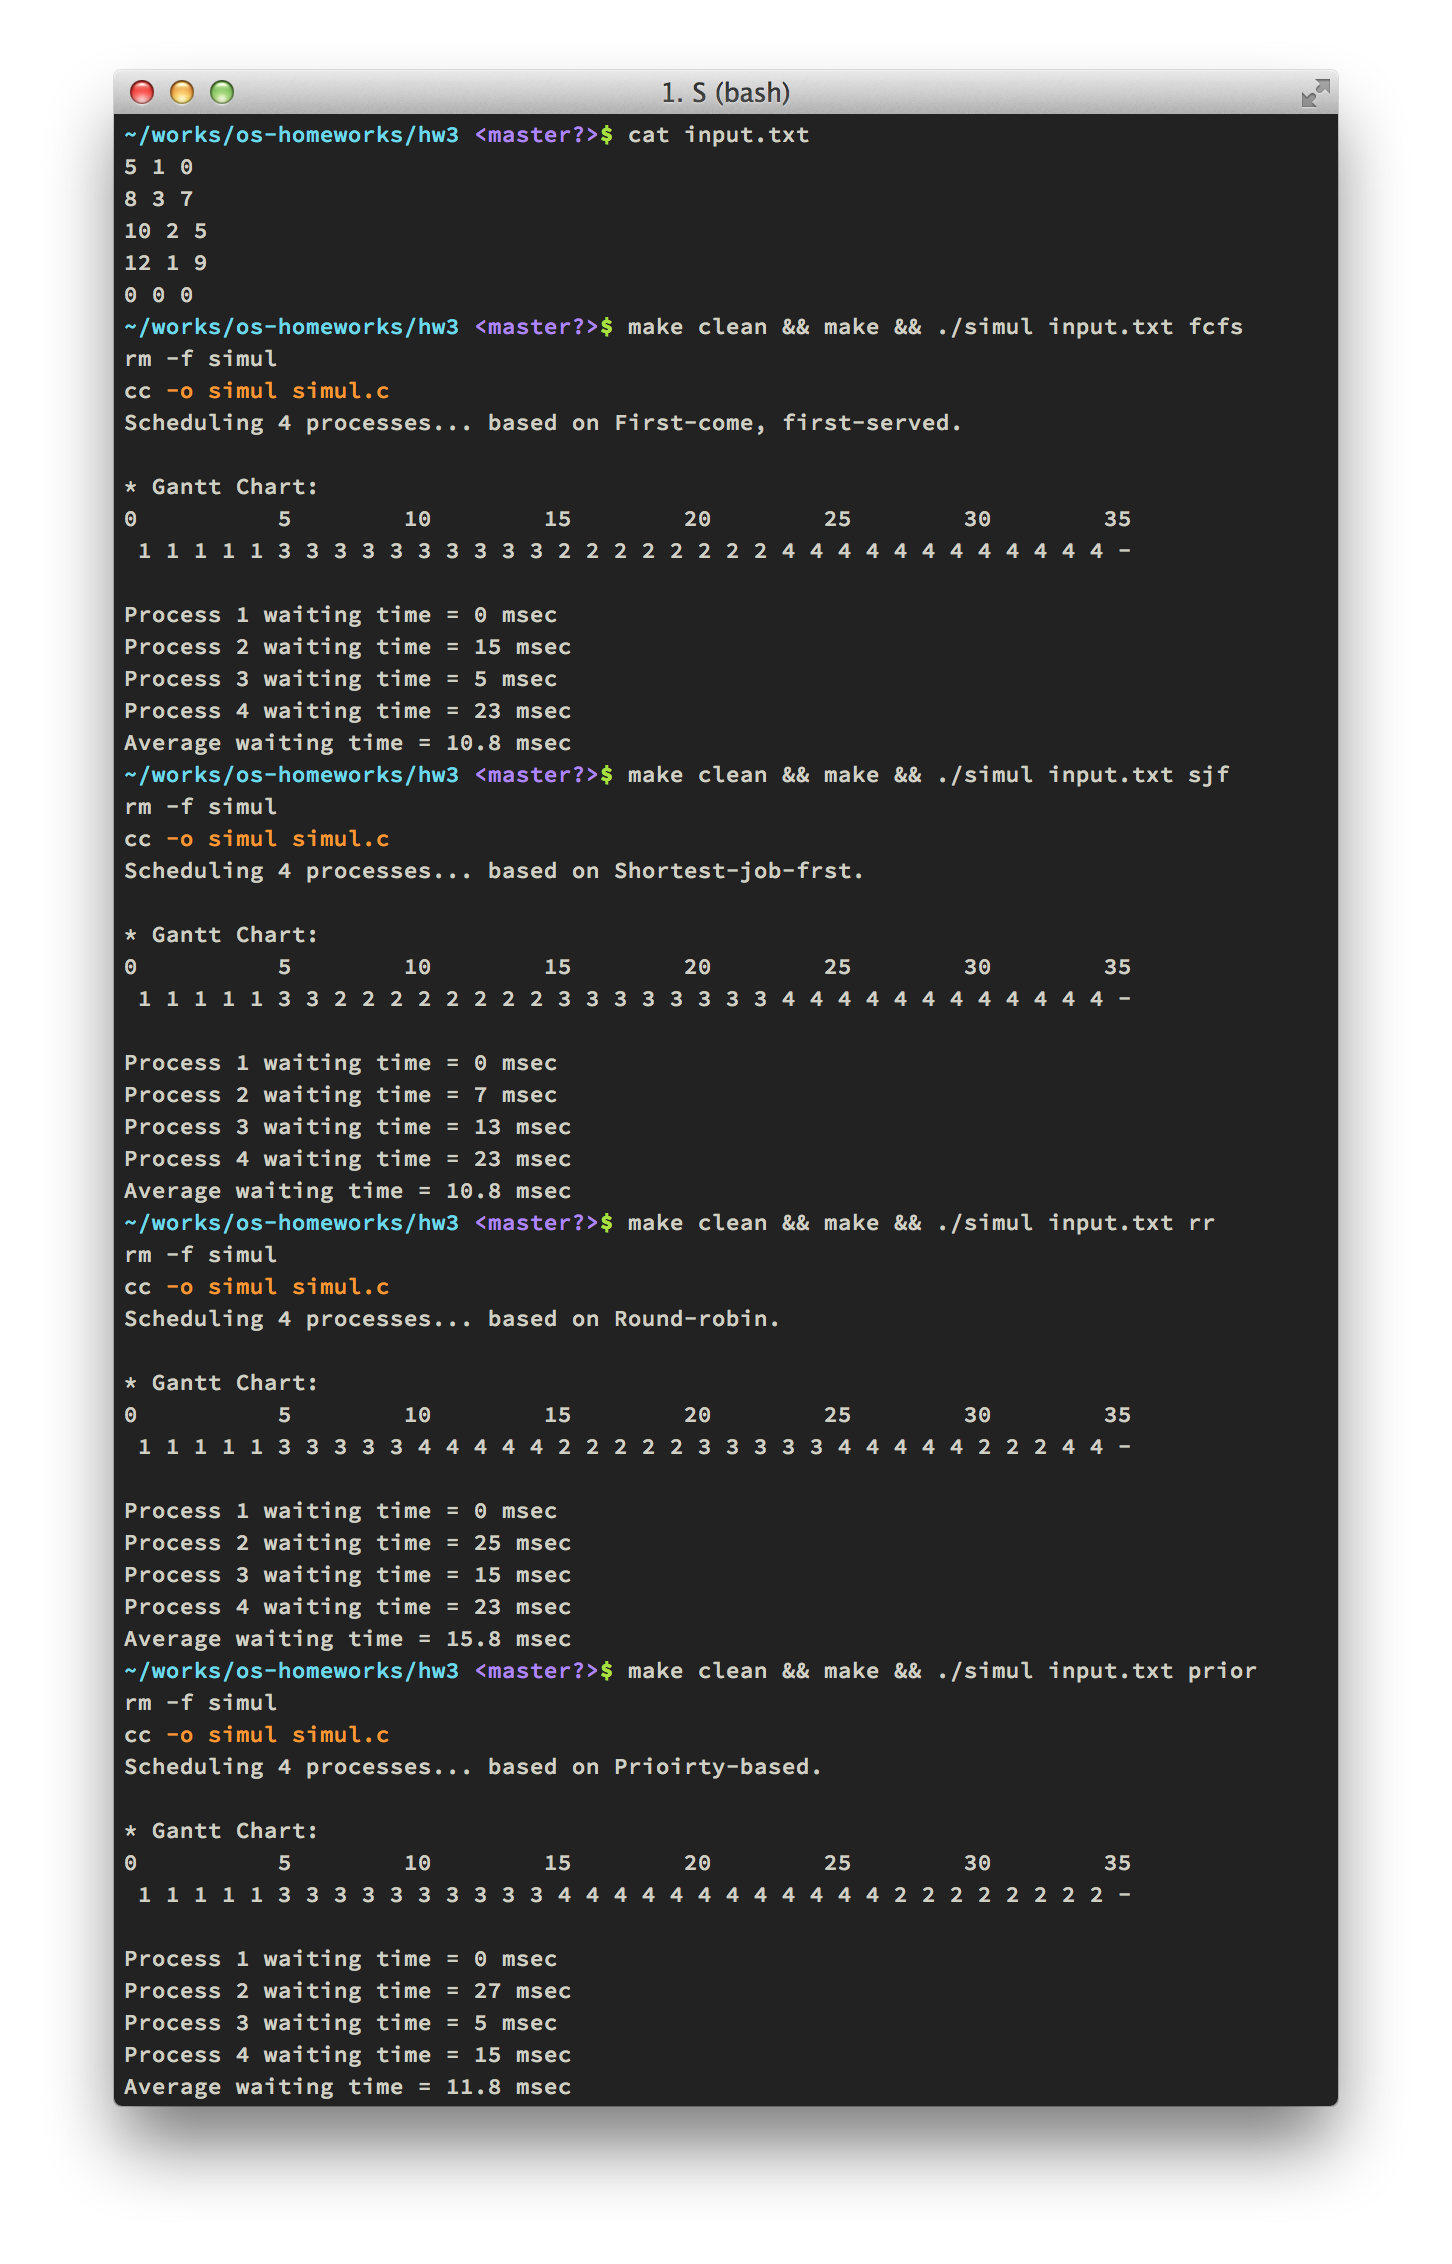
\includegraphics[width=\textwidth]{screenshot.png}

\subsection*{Source codes:}

\subsubsection*{Makefile}
\inputminted[fontsize=\footnotesize,linenos]{basemake}{Makefile}

\subsubsection*{simul.c (Main source code)}
\inputminted[fontsize=\footnotesize,linenos]{c}{simul.c}

\end{document}
